% ============================================================
% f2013_tianjin_science_q13_circle.tex
% 2013 天津卷（理科）第 13 题 圆内接三角形与切线（TikZ 矢量重绘）
% 几何：圆 O，A 在圆上；AB=AC；BD∥AC，E 在 DB 延长线上，EA 切圆于 A；
%       AD 与 BC 交于 F。图中坐标按题设 AE=6、BD=5、AB=AC 精确构造后缩放。
% ============================================================
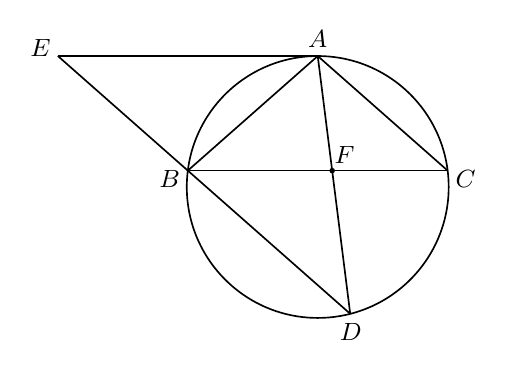
\begin{tikzpicture}[
  x=1cm, y=1cm,
  every node/.style={font=\small, inner sep=1pt},
  line/.style={line width=0.6pt},
]

  % 圆：R = 8/sqrt(7) * 0.55
  \draw[line] (0,0) circle [radius=1.6630];

  % 切线 EA 与割线 E-B-D
  \draw[line] (-3.30,1.6630) -- (0,1.6630);
  \draw[line] (-3.30,1.6630) -- (0.4125,-1.6105);

  % 三角形 ABC 与弦 AD
  \draw[line] (0,1.6630) -- (-1.6500,0.2078);
  \draw[line] (0,1.6630) -- (1.6500,0.2078);
  \draw[line] (-1.6500,0.2078) -- (1.6500,0.2078);
  \draw[line] (0,1.6630) -- (0.4125,-1.6105);

  % 交点 F
  \fill (0.1833,0.2078) circle [radius=0.035];

  % 标签
  \node at (0,1.88) {$A$};
  \node at (-1.88,0.10) {$B$};
  \node at (1.88,0.10) {$C$};
  \node at (0.42,-1.84) {$D$};
  \node at (-3.52,1.76) {$E$};
  \node at (0.34,0.40) {$F$};

\end{tikzpicture}
